\documentclass[border=10pt,tikz]{standalone}
\usepackage{pgfplots}
\usepackage{amsmath, amssymb, amsfonts}
\usetikzlibrary{calc}
\usepgfplotslibrary{fillbetween}
% \usepackage{pgfplotstable}
\def\axisdefaultwidth{15cm}
\def\axisdefaultheight{5cm}
\begin{document}
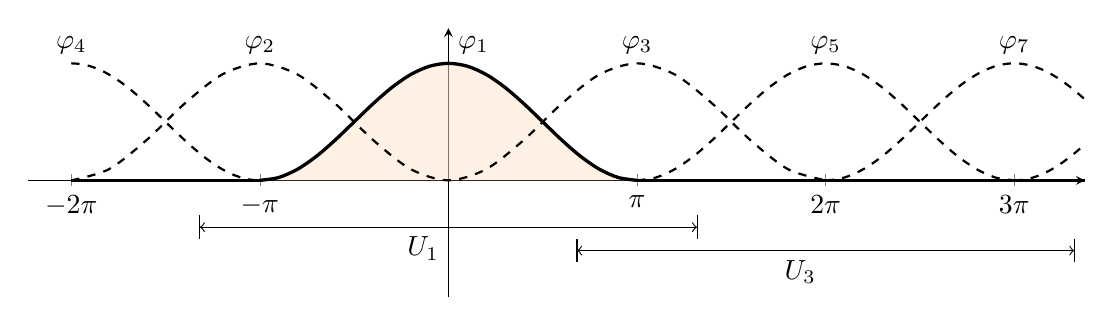
\begin{tikzpicture}
  \begin{axis} [
    xmin = -7, xmax=10.6,
    ymin = -1, ymax = 1.3,
    axis lines = middle,
    xtick = {-2*pi, -pi, 0, pi, 2*pi, 3*pi},
    xticklabels = {$-2\pi$, $-\pi$, $0$, $\pi$, $2\pi$, $3\pi$ },
    ytick = \empty
    ]
    \addplot [name path = p1, domain=-pi:pi, smooth, very thick, samples=21]{(1+cos (deg(x)))/2 };
    \addplot [domain=-2*pi:-pi, smooth, very thick, samples=21]{0*x };
    \addplot [domain=pi:10.6, smooth, very thick, samples=21]{0*x };
    \addplot [name path = p2, domain=-2*pi:2*pi, smooth, thick, dashed, samples=21]{(1+cos (deg(x+pi)))/2 };
    \addplot [name path = p3, domain=-2*pi:-pi, smooth, thick, dashed, samples=21]{(1+cos (deg(x+2*pi)))/2 };
    \addplot [name path = p4, domain=pi:3*pi, smooth, thick, dashed, samples=21]{(1+cos (deg(x-2*pi)))/2 };
    \addplot [name path = p5, domain=2*pi:10.6, smooth, thick, dashed, samples=21]{(1+cos (deg(x-3*pi)))/2 };
    \addplot [name path = p5, domain=3*pi:10.6, smooth, thick, dashed, samples=21]{(1+cos (deg(x-4*pi)))/2 };

    \path [name path = axis] (axis cs:-2*pi,0) -- (axis cs:3*pi,0);

    \addplot [orange!20, opacity=0.5] fill between [of=p1 and axis];
    
    \draw[] (axis cs: -pi-1, -0.30) -- (axis cs: -pi-1, -0.5);
    \draw[] (axis cs: pi+1, -0.3) -- (axis cs: pi+1, -0.5);
    \draw[<->] (axis cs: -pi-1, -0.4) --node[below left] {$U_1$} (axis cs: pi+1, -0.4);
    
    \draw[] (axis cs: pi-1, -0.50) -- (axis cs: pi-1, -0.7);
    \draw[] (axis cs: 3*pi+1, -0.5) -- (axis cs: 3*pi+1, -0.7);
    \draw[<->] (axis cs: pi-1, -0.6) --node[below left] {$U_3$} (axis cs: 3*pi+1, -0.6);

    \node[above] at (axis cs:pi, 1) {$\varphi_3$};
    \node[above right] at (axis cs:0, 1) {$\varphi_1$};
    \node[above] at (axis cs:-pi, 1) {$\varphi_2$};
    \node[above] at (axis cs:-2*pi, 1) {$\varphi_4$};
    \node[above] at (axis cs:2*pi, 1) {$\varphi_5$};
    \node[above] at (axis cs:3*pi, 1) {$\varphi_7$};
  \end{axis}
\end{tikzpicture}
\end{document} 



